\documentclass[tikz,border=1pt]{standalone}
\usepackage[T1]{fontenc}
\usepackage{times}
\usepackage{amsmath,amssymb}
% Shared visual language for Figures 1 and 2 (flat illustration style, serif labels).
\usetikzlibrary{arrows.meta,calc,positioning,shadows.blur,decorations.pathreplacing,backgrounds,fit}

% ---------------------------------------------------------------- palette (shared with Figure 2)
% Light, low-saturation fills; hairline frames in the same hue; one semantic colour per role.
\definecolor{ink}{HTML}{263040}
\definecolor{ink2}{HTML}{667085}
\definecolor{icon}{HTML}{4B5565}     % icon strokes
\definecolor{line}{HTML}{D0D7E2}
\definecolor{paper}{HTML}{FFFFFF}
\definecolor{bookcov}{HTML}{A9B9CF}
% panel families (frame / header band / body): white panels, grey hairline frames
\definecolor{pblue}{HTML}{D3D9E2}      \definecolor{pbluehead}{HTML}{FFFFFF}   \definecolor{pbluebg}{HTML}{FFFFFF}
\definecolor{porange}{HTML}{D3D9E2}    \definecolor{porangehead}{HTML}{FFFFFF} \definecolor{porangebg}{HTML}{FFFFFF}
\definecolor{pmist}{HTML}{D3D9E2}      \definecolor{pmisthead}{HTML}{FFFFFF}   \definecolor{pmistbg}{HTML}{FFFFFF}
% semantic accents
\definecolor{hind}{HTML}{3D7FD9}     % teacher prediction f_k (blue)
\definecolor{hindbg}{HTML}{E6F0FC}
\definecolor{sage}{HTML}{7B68D6}     % verified forks, Y-hat (lavender)
\definecolor{sagebg}{HTML}{F4F2FD}
\definecolor{sagecard}{HTML}{ECE8FB}
\definecolor{ok}{HTML}{3D7FD9}       % verified success (blue)
\definecolor{bad}{HTML}{E06C5F}      % failure, slip, blame (coral)
\definecolor{badbg}{HTML}{FDECEA}
\definecolor{gold}{HTML}{F2B27A}     % agreement highlight (apricot)
\definecolor{ours}{HTML}{E8894A}     % credit / update accent (apricot)
% credit bars, same tints as the tokens of Figure 2
\definecolor{tokbluetop}{HTML}{DCEAFB} \definecolor{tokbluebot}{HTML}{BCD6F5} \definecolor{tokblueln}{HTML}{6F9BD8}
\definecolor{tokredtop}{HTML}{FBDAD5}  \definecolor{tokredbot}{HTML}{F4B5AC}  \definecolor{tokredln}{HTML}{D9685C}
\colorlet{coral}{pmist}\colorlet{coralbg}{pmistbg}\colorlet{coralcard}{white}

\tikzset{
  >={Stealth[length=4.2pt,width=3.6pt]},
  base/.style={font=\fontsize{7.3}{8.8}\selectfont, text=ink},
  arr/.style={->, line width=0.75pt, draw=ink},
  arrsoft/.style={->, line width=0.7pt, draw=ink2},
  card/.style={rounded corners=4pt, line width=0.55pt},
  chip/.style={rounded corners=2.5pt, line width=0.65pt, minimum height=0.46cm, minimum width=0.62cm, inner sep=1.5pt, font=\fontsize{7.6}{9}\selectfont},
  lab/.style={font=\fontsize{7.3}{8.6}\selectfont, text=ink, align=center},
  small/.style={font=\fontsize{6.7}{7.8}\selectfont, text=ink2, align=center},
  ttl/.style={font=\fontsize{7.8}{9.2}\selectfont\bfseries, text=ink, align=left},
  % ------------------------------------------------------------ icons
  doc/.pic={
    \draw[icon, fill=paper, line width=0.65pt, line join=round]
      (-0.32,-0.42) -- (0.32,-0.42) -- (0.32,0.28) -- (0.18,0.42) -- (-0.32,0.42) -- cycle;
    \draw[icon, line width=0.6pt, line join=round] (0.18,0.42) -- (0.18,0.28) -- (0.32,0.28);
    \foreach \y in {0.17,0.04,-0.09,-0.22} \draw[icon!40, line width=0.6pt, line cap=round] (-0.2,\y) -- (0.19,\y);
  },
  % a document whose third line carries a slip (wrong turn)
  docslip/.pic={
    \draw[icon, fill=paper, line width=0.65pt, line join=round]
      (-0.32,-0.42) -- (0.32,-0.42) -- (0.32,0.28) -- (0.18,0.42) -- (-0.32,0.42) -- cycle;
    \draw[icon, line width=0.6pt, line join=round] (0.18,0.42) -- (0.18,0.28) -- (0.32,0.28);
    \foreach \y in {0.17,0.04,-0.22} \draw[icon!40, line width=0.6pt, line cap=round] (-0.2,\y) -- (0.19,\y);
    \draw[bad, line width=1.1pt, line cap=round] (-0.2,-0.09) -- (0.19,-0.09);
    \draw[bad, line width=1.0pt, line cap=round] (0.05,-0.02) -- (0.24,0.22);
  },
  % a document with highlighted (reference-like) lines
  dochl/.pic={
    \draw[icon, fill=paper, line width=0.65pt, line join=round] (-0.32,-0.42) -- (0.32,-0.42) -- (0.32,0.28) -- (0.18,0.42) -- (-0.32,0.42) -- cycle;
    \draw[icon, line width=0.6pt, line join=round] (0.18,0.42) -- (0.18,0.28) -- (0.32,0.28);
    \fill[gold!45] (-0.23,0.11) rectangle (0.22,0.23);
    \fill[gold!45] (-0.23,-0.02) rectangle (0.22,0.10);
    \foreach \y in {0.17,0.04,-0.09,-0.22} \draw[icon!40, line width=0.6pt, line cap=round] (-0.2,\y) -- (0.19,\y);
  },
  book/.pic={
    \fill[bookcov, rounded corners=1pt] (-0.62,-0.34) -- (0,-0.40) -- (0.62,-0.34) -- (0.62,0.30) -- (0,0.24) -- (-0.62,0.30) -- cycle;
    \draw[icon, fill=paper, line width=0.65pt, line join=round] (-0.58,0.36) .. controls (-0.3,0.40) and (-0.12,0.36) .. (0,0.28) -- (0,-0.32) .. controls (-0.12,-0.25) and (-0.3,-0.22) .. (-0.58,-0.26) -- cycle;
    \draw[icon, fill=paper, line width=0.65pt, line join=round] (0.58,0.36) .. controls (0.3,0.40) and (0.12,0.36) .. (0,0.28) -- (0,-0.32) .. controls (0.12,-0.25) and (0.3,-0.22) .. (0.58,-0.26) -- cycle;
    \foreach \y in {0.18,0.06,-0.06,-0.16} {
      \draw[icon!40, line width=0.55pt, line cap=round] (-0.48,\y+0.03) .. controls (-0.3,\y+0.05) .. (-0.1,\y);
      \draw[icon!40, line width=0.55pt, line cap=round] (0.48,\y+0.03) .. controls (0.3,\y+0.05) .. (0.1,\y);
    }
  },
  clipboard/.pic={
    \draw[icon, fill=paper, line width=0.7pt, rounded corners=2pt] (-0.34,-0.45) rectangle (0.34,0.38);
    \draw[icon, fill=icon!55, line width=0.6pt, rounded corners=1.5pt] (-0.15,0.31) rectangle (0.15,0.46);
    \fill[icon!55] (0,0.49) circle (0.045);
  },
  xmark/.pic={\draw[bad, line width=1.6pt, line cap=round] (-0.15,-0.15) -- (0.15,0.15) (-0.15,0.15) -- (0.15,-0.15);},
  badx/.pic={\fill[bad] (0,0) circle (0.15); \draw[white, line width=1.1pt, line cap=round] (-0.065,-0.065) -- (0.065,0.065) (-0.065,0.065) -- (0.065,-0.065);},
  badok/.pic={\fill[ok] (0,0) circle (0.15); \draw[white, line width=1.1pt, line cap=round, line join=round] (-0.075,0.0) -- (-0.02,-0.06) -- (0.08,0.07);},
  magnifier/.pic={
    \draw[icon, line width=1.6pt, line cap=round] (0.15,-0.15) -- (0.36,-0.36);
    \draw[icon, fill=hindbg, fill opacity=0.85, line width=0.9pt] (0,0) circle (0.21);
  },
  eye/.pic={
    \draw[icon, fill=paper, line width=0.7pt] (-0.36,0) .. controls (-0.14,0.26) and (0.14,0.26) .. (0.36,0) .. controls (0.14,-0.26) and (-0.14,-0.26) .. (-0.36,0) -- cycle;
    \fill[hind] (0,0) circle (0.12); \fill[icon] (0,0) circle (0.055); \fill[white] (0.035,0.04) circle (0.025);
  },
  dice/.pic={
    \draw[icon, fill=paper, line width=0.7pt, rounded corners=2.5pt] (-0.22,-0.22) rectangle (0.22,0.22);
    \foreach \p in {(-0.11,0.11),(0.11,-0.11),(0,0),(-0.11,-0.11),(0.11,0.11)} \fill[icon] \p circle (0.035);
  },
  snow/.pic={
    \foreach \a in {0,60,120} \draw[white, line width=0.9pt, line cap=round] (\a:0.16) -- (\a+180:0.16);
    \foreach \a in {0,60,...,300} \draw[white, line width=0.6pt, line cap=round] (\a:0.1) -- ++(\a+40:0.05) (\a:0.1) -- ++(\a-40:0.05);
  },
  robot/.pic={
    \draw[icon, line width=0.7pt] (0,0.52) -- (0,0.66); \fill[ours] (0,0.69) circle (0.06);
    \draw[icon, fill=paper, line width=0.75pt, rounded corners=4pt] (-0.40,0.05) rectangle (0.40,0.54);
    \draw[icon, fill=paper, line width=0.6pt, rounded corners=1pt] (-0.47,0.20) rectangle (-0.40,0.38) (0.40,0.20) rectangle (0.47,0.38);
    \fill[icon] (-0.15,0.31) circle (0.065) (0.15,0.31) circle (0.065);
    \draw[icon, line width=0.6pt, line cap=round] (-0.1,0.15) -- (0.1,0.15);
    \draw[icon, fill=tokblueln!75, line width=0.75pt, rounded corners=4pt] (-0.46,-0.52) rectangle (0.46,0.0);
    \pic at (0,-0.26) {snow};
  },
  gauge/.pic={
    \draw[line, line width=3.2pt] (180:0.38) arc (180:0:0.38);
    \draw[sage!80, line width=3.2pt] (180:0.38) arc (180:115:0.38);
    \draw[icon, line width=1.0pt, line cap=round] (0,0) -- (118:0.33);
    \fill[icon] (0,0) circle (0.05);
  },
  slider/.pic={
    \draw[line, line width=2.4pt, line cap=round] (0,0) -- (1.5,0);
    \draw[ours, line width=2.4pt, line cap=round] (0,0) -- (1.2,0);
    \draw[icon, fill=paper, line width=0.8pt] (1.2,0) circle (0.11);
  },
  scales/.pic={
    \draw[icon, line width=0.8pt, line cap=round] (0,-0.32) -- (0,0.26) (-0.18,-0.32) -- (0.18,-0.32) (-0.38,0.2) -- (0.38,0.2);
    \fill[icon] (0,0.29) circle (0.05);
    \draw[icon, line width=0.55pt] (-0.38,0.2) -- (-0.5,-0.04) (-0.38,0.2) -- (-0.26,-0.04) (0.38,0.2) -- (0.26,-0.04) (0.38,0.2) -- (0.5,-0.04);
    \draw[icon, fill=hindbg, line width=0.65pt] (-0.52,-0.04) arc (180:360:0.14);
    \draw[icon, fill=sagecard, line width=0.65pt] (0.24,-0.04) arc (180:360:0.14);
  },
  refresh/.pic={
    \draw[sage, line width=1.1pt, ->] (60:0.2) arc (60:330:0.2);
  },
}

% panel in the style of Figure 2: hairline frame, light header band, dark bold title
% #1 name, #2 frame colour (header colour is #2head), #3 body colour, #4 sw corner, #5 ne corner, #6 title
\newcommand{\panel}[6]{%
  \path[fill=#3, rounded corners=5pt] (#4) rectangle (#5);
  \begin{scope}
    \clip[rounded corners=5pt] (#4) rectangle (#5);
    \fill[#2head] ($(#4|-#5)+(0,-0.56)$) rectangle (#5);
    \draw[#2, line width=0.5pt] ($(#4|-#5)+(0,-0.56)$) -- ($(#5)+(0,-0.56)$);
  \end{scope}
  \draw[#2, line width=0.75pt, rounded corners=5pt] (#4) rectangle (#5);
  \node[anchor=center, text=ink, font=\fontsize{8.4}{10}\selectfont\bfseries] at ($($(#4|-#5)!0.5!(#5)$)+(0,-0.28)$) {#6};
}

\tikzset{
  calib/.pic={
    \draw[icon, fill=paper, line width=0.7pt, rounded corners=2.5pt] (-0.36,-0.32) rectangle (0.36,0.32);
    \foreach \y/\k in {0.16/0.12,0.0/-0.1,-0.16/0.06} {
      \draw[line, line width=1.2pt, line cap=round] (-0.24,\y) -- (0.24,\y);
      \fill[hind] (\k,\y) circle (0.055);
    }
  },
  feats/.pic={
    \foreach \x/\h [count=\i] in {-0.24/0.22,-0.12/0.36,0/0.15,0.12/0.3,0.24/0.2} \fill[hind!60, rounded corners=0.6pt] (\x-0.045,-0.2) rectangle (\x+0.045,-0.2+\h);
    \draw[ink2, line width=0.5pt] (-0.32,-0.2) -- (0.32,-0.2);
  },
  fold/.pic={
    \draw[icon, fill=paper, line width=0.6pt, rounded corners=1.5pt] (-0.2,-0.24) rectangle (0.2,0.24);
    \foreach \y in {0.11,0.0,-0.11} \draw[icon!40, line width=0.5pt] (-0.12,\y) -- (0.12,\y);
  },
}

\tikzset{
  robotlive/.pic={
    \draw[icon, line width=0.7pt] (0,0.52) -- (0,0.66); \fill[ours] (0,0.69) circle (0.06);
    \draw[icon, fill=paper, line width=0.75pt, rounded corners=4pt] (-0.40,0.05) rectangle (0.40,0.54);
    \draw[icon, fill=paper, line width=0.6pt, rounded corners=1pt] (-0.47,0.20) rectangle (-0.40,0.38) (0.40,0.20) rectangle (0.47,0.38);
    \fill[icon] (-0.15,0.31) circle (0.065) (0.15,0.31) circle (0.065);
    \draw[icon, line width=0.6pt, line cap=round] (-0.12,0.16) .. controls (-0.04,0.1) and (0.04,0.1) .. (0.12,0.16);
    \draw[icon, fill=ours!55, line width=0.75pt, rounded corners=4pt] (-0.46,-0.52) rectangle (0.46,0.0);
    \draw[white, line width=1.0pt, ->, >={Stealth[length=2.8pt,width=2.6pt]}] (60:0.15)++(0,-0.26) arc (60:330:0.15);
  },
  foldlab/.pic={
    \draw[icon, fill=paper, line width=0.6pt, rounded corners=1.5pt] (-0.21,-0.25) rectangle (0.21,0.25);
  },
}


% ---------------------------------------------------------------- colours shared with Figure 2
\definecolor{tbT}{HTML}{BCDFF5}\definecolor{tbS}{HTML}{94C1E5}\definecolor{tbL}{HTML}{344858}   % before the slip
\definecolor{trT}{HTML}{F5AEA9}\definecolor{trS}{HTML}{E89591}\definecolor{trL}{HTML}{AD4E33}   % the slip
\definecolor{taT}{HTML}{FFDCAD}\definecolor{taS}{HTML}{F5C98E}\definecolor{taL}{HTML}{A36736}   % after the slip
\definecolor{docb}{HTML}{EEF6FD}\definecolor{docr}{HTML}{FDEEEC}\definecolor{doca}{HTML}{FFF5E8}  % document tints
\definecolor{panelbg}{HTML}{EEF1F6}
\definecolor{robotbody}{HTML}{9CC3EA}

\tikzset{
  title/.style={font=\fontsize{8.4}{10}\selectfont\bfseries, text=ink, anchor=west},
  sub/.style={font=\fontsize{7.4}{9}\selectfont\bfseries, text=ink, anchor=west},
  pill/.style={draw=line, fill=white, rounded corners=2pt, line width=0.5pt, minimum width=0.6cm, minimum height=0.3cm, inner sep=0pt},
  softcard/.style={fill=white, rounded corners=5pt},   % white card on the grey panel: no stroke, no shadow
}
% panel: borderless soft background, title inside
\newcommand{\panelbg}[5]{%
  \path[fill=panelbg, rounded corners=7pt] (#1,#2) rectangle (#3,#4);
  \node[title] at (#1+0.22,#4-0.36) {#5};
}
% document icon tinted with the colour of its segment: x, y, scale, tint
\newcommand{\docat}[4]{%
  \begin{scope}[shift={(#1,#2)}, scale=#3]
    \draw[icon, fill=#4, line width=0.6pt, line join=round] (-0.32,-0.42) -- (0.32,-0.42) -- (0.32,0.28) -- (0.18,0.42) -- (-0.32,0.42) -- cycle;
    \draw[icon, fill=white, line width=0.55pt, line join=round] (0.18,0.42) -- (0.18,0.28) -- (0.32,0.28) -- cycle;
    \foreach \y in {0.17,0.04,-0.09,-0.22} \draw[icon!40, line width=0.6pt, line cap=round] (-0.2,\y) -- (0.19,\y);
  \end{scope}}
% the document with the slip: a struck line and a pen mark
\newcommand{\docslipat}[3]{%
  \begin{scope}[shift={(#1,#2)}, scale=#3]
    \draw[icon, fill=docr, line width=0.6pt, line join=round] (-0.32,-0.42) -- (0.32,-0.42) -- (0.32,0.28) -- (0.18,0.42) -- (-0.32,0.42) -- cycle;
    \draw[icon, fill=white, line width=0.55pt, line join=round] (0.18,0.42) -- (0.18,0.28) -- (0.32,0.28) -- cycle;
    \foreach \y in {0.17,0.04,-0.22} \draw[icon!40, line width=0.6pt, line cap=round] (-0.2,\y) -- (0.19,\y);
    \draw[bad, line width=1.1pt, line cap=round] (-0.2,-0.09) -- (0.19,-0.09);
    \draw[bad, line width=1.0pt, line cap=round] (0.05,-0.02) -- (0.24,0.22);
  \end{scope}}
% small robot: the frozen policy pi_old
\newcommand{\robotat}[3]{%
  \begin{scope}[shift={(#1,#2)}, scale=#3]
    \draw[icon, line width=0.7pt] (0,0.52) -- (0,0.66); \fill[hind] (0,0.69) circle (0.06);
    \draw[icon, fill=white, line width=0.7pt, rounded corners=4pt] (-0.40,0.05) rectangle (0.40,0.54);
    \draw[icon, fill=white, line width=0.6pt, rounded corners=1pt] (-0.47,0.20) rectangle (-0.40,0.38) (0.40,0.20) rectangle (0.47,0.38);
    \fill[icon] (-0.15,0.31) circle (0.065) (0.15,0.31) circle (0.065);
    \draw[icon, line width=0.6pt, line cap=round] (-0.1,0.15) -- (0.1,0.15);
    \draw[icon, fill=robotbody, line width=0.7pt, rounded corners=4pt] (-0.46,-0.52) rectangle (0.46,0.0);
    \pic at (0,-0.26) {snow};
  \end{scope}}
% credit bar: family, x, signed height
\newcommand{\creditbar}[3]{%
  \shade[top color=t#1T, bottom color=t#1S, rounded corners=0.8pt] (#2-0.19,0) rectangle (#2+0.19,#3);
  \draw[t#1L, line width=0.5pt, rounded corners=0.8pt] (#2-0.19,0) rectangle (#2+0.19,#3);
}

\begin{document}
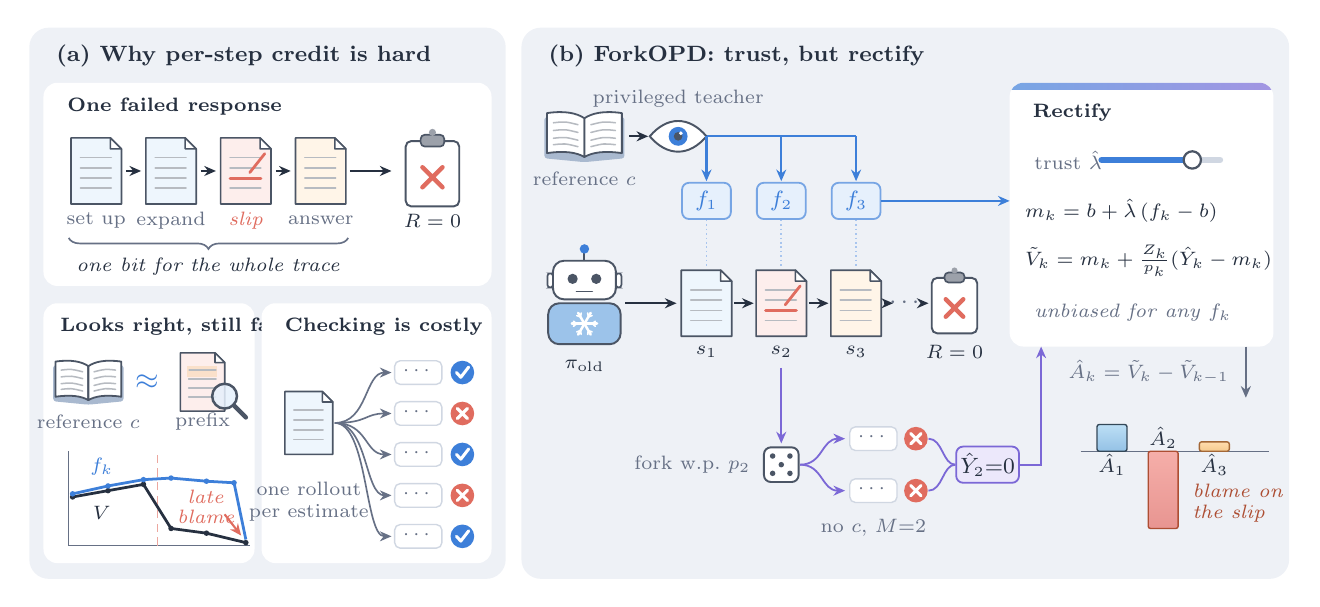
\begin{tikzpicture}[base]

% =================================================================== two panels of equal height
\panelbg{0}{0}{6.05}{7.0}{(a)~Why per-step credit is hard}
\panelbg{6.25}{0}{16.0}{7.0}{(b)~ForkOPD: trust, but rectify}

% =================================================================== (a) card 1: one failed response
\path[softcard] (0.18,3.72) rectangle (5.87,6.3);
\node[sub] at (0.36,6.0) {One failed response};
\docat{0.85}{5.18}{1.0}{docb}
\docat{1.8}{5.18}{1.0}{docb}
\docslipat{2.75}{5.18}{1.0}
\docat{3.7}{5.18}{1.0}{doca}
\foreach \x in {0.85,1.8,2.75} \draw[arr] (\x+0.38,5.18) -- (\x+0.57,5.18);
\foreach \x/\l in {0.85/set up,1.8/expand,3.7/answer} \node[small] at (\x,4.55) {\l};
\node[small, text=bad, font=\fontsize{6.7}{7.8}\selectfont\itshape] at (2.75,4.55) {slip};
\draw[arr] (4.07,5.18) -- (4.6,5.18);
\pic[scale=1.0] at (5.12,5.18) {clipboard};
\pic[scale=0.85] at (5.12,5.1) {xmark};
\node[lab] at (5.12,4.55) {$R=0$};
\draw[decorate, decoration={brace, mirror, amplitude=4pt}, line width=0.6pt, ink2] (0.5,4.33) -- (4.05,4.33);
\node[lab, font=\fontsize{7.3}{8.6}\selectfont\itshape] at (2.27,3.97) {one bit for the whole trace};

% =================================================================== (a) card 2: looks right, still fails
\path[softcard] (0.18,0.2) rectangle (2.86,3.5);
\node[sub] at (0.27,3.2) {Looks right, still fails};
\pic[scale=0.72] at (0.75,2.5) {book};
\node[small] at (0.75,2.0) {reference $c$};
\node[text=hind, font=\fontsize{11}{11}\selectfont\bfseries] at (1.5,2.5) {$\approx$};
\docat{2.2}{2.5}{0.88}{docr}
\fill[gold!40] (2.2-0.2,2.5+0.06) rectangle (2.2+0.19,2.5+0.2);
\foreach \y in {0.15,0.035} \draw[icon!40, line width=0.55pt, line cap=round] (2.2-0.17,2.5+\y) -- (2.2+0.17,2.5+\y);
\pic[scale=0.75] at (2.48,2.32) {magnifier};
\node[small] at (2.2,2.0) {prefix};
\begin{scope}[shift={(0.5,0.42)}]
  \draw[ink2, line width=0.5pt] (0,0) -- (2.3,0);
  \draw[ink2, line width=0.5pt] (0,0) -- (0,1.2);
  \draw[bad!60, densely dashed, line width=0.5pt] (1.13,0) -- (1.13,1.15);
  \draw[ink, line width=1.0pt, line join=round] (0.05,0.62) -- (0.5,0.7) -- (0.95,0.78) -- (1.3,0.22) -- (1.75,0.16) -- (2.25,0.04);
  \draw[hind, line width=1.0pt, line join=round] (0.05,0.66) -- (0.5,0.76) -- (0.95,0.84) -- (1.3,0.86) -- (1.75,0.82) -- (2.1,0.8) -- (2.25,0.08);
  \foreach \p in {(0.05,0.62),(0.5,0.7),(0.95,0.78),(1.3,0.22),(1.75,0.16),(2.25,0.04)} \fill[ink] \p circle (0.035);
  \foreach \p in {(0.05,0.66),(0.5,0.76),(0.95,0.84),(1.3,0.86),(1.75,0.82),(2.1,0.8)} \fill[hind] \p circle (0.035);
  \node[font=\fontsize{6.8}{7}\selectfont, text=hind] at (0.42,1.0) {$f_k$};
  \node[font=\fontsize{6.8}{7}\selectfont, text=ink] at (0.42,0.42) {$V$};
  \node[font=\fontsize{6.7}{7.2}\selectfont\itshape, text=bad, align=center] at (1.74,0.5) {late\\blame};
  \draw[bad, line width=0.75pt, ->] (1.98,0.4) -- (2.19,0.13);
\end{scope}

% =================================================================== (a) card 3: checking is costly
\path[softcard] (2.95,0.2) rectangle (5.87,3.5);
\node[sub] at (3.12,3.2) {Checking is costly};
\docat{3.55}{1.98}{0.95}{docb}
\foreach \y/\m [count=\i] in {2.62,2.1,1.58,1.06,0.54} {
  \ifnum\i=2 \def\mm{badx}\else\ifnum\i=4 \def\mm{badx}\else\def\mm{badok}\fi\fi
  \draw[ink2, line width=0.6pt, ->] (3.88,1.98) .. controls (4.3,1.98) and (4.26,\y) .. (4.6,\y);
  \node[pill] at (4.94,\y) {}; \node[font=\fontsize{6.7}{6.7}\selectfont, text=ink2] at (4.94,\y+0.02) {$\cdots$};
  \pic at (5.5,\y) {\mm};
}
\node[small, align=center] at (3.55,0.98) {one rollout\\per estimate};

% =================================================================== (b) privileged teacher (top row)
\pic[scale=0.82] at (7.05,5.62) {book};
\node[small] at (7.05,5.08) {reference $c$};
\draw[arr] (7.62,5.62) -- (7.86,5.62);
\pic at (8.24,5.62) {eye};
\node[small, anchor=south] at (8.24,5.86) {privileged teacher};
\draw[hind, line width=0.75pt] (8.61,5.62) -- (10.5,5.62);
\foreach \x [count=\i] in {8.6,9.55,10.5} {
  \draw[hind, line width=0.75pt, ->] (\x,5.62) -- (\x,5.05);
  \node[chip, draw=hind!70, fill=hindbg, text=hind] (f\i) at (\x,4.8) {$f_{\i}$};
  \draw[hind!45, densely dotted, line width=0.6pt] (\x,4.56) -- (\x,3.95);
}

% =================================================================== (b) the sampled response (middle row)
\def\ry{3.5}
\robotat{7.05}{\ry}{1.0}
\node[lab] at (7.05,\ry-0.8) {$\pi_{\mathrm{old}}$};
\draw[arr] (7.57,\ry) -- (8.22,\ry);
\docat{8.6}{\ry}{1.0}{docb}
\docslipat{9.55}{\ry}{1.0}
\docat{10.5}{\ry}{1.0}{doca}
\draw[arr] (8.95,\ry) -- (9.2,\ry);
\draw[arr] (9.9,\ry) -- (10.15,\ry);
\draw[arr] (10.85,\ry) -- (10.97,\ry);
\node[font=\fontsize{9}{9}\selectfont, text=ink2] at (11.14,\ry) {$\cdots$};
\draw[arr] (11.32,\ry) -- (11.42,\ry);
\pic[scale=0.85] at (11.75,\ry) {clipboard};
\pic[scale=0.74] at (11.75,\ry-0.06) {xmark};
\node[lab] at (11.75,\ry-0.62) {$R=0$};
\foreach \x [count=\i] in {8.6,9.55,10.5} \node[lab] at (\x,\ry-0.62) {$s_{\i}$};

% =================================================================== (b) random fork at s_2 (bottom row)
\def\fy{1.45}
\draw[arr, draw=sage] (9.55,\ry-0.82) -- (9.55,\fy+0.27);
\pic at (9.55,\fy) {dice};
\node[small, anchor=east] at (9.28,\fy) {fork w.p.\ $p_2$};
\foreach \y in {\fy+0.33,\fy-0.33} {
  \draw[sage, line width=0.65pt, ->] (9.79,\fy) .. controls (10.08,\fy) and (10.06,\y) .. (10.36,\y);
  \node[pill] at (10.72,\y) {}; \node[font=\fontsize{6.7}{6.7}\selectfont, text=ink2] at (10.72,\y+0.02) {$\cdots$};
  \pic at (11.26,\y) {badx};
  \draw[sage, line width=0.65pt] (11.42,\y) .. controls (11.6,\y) and (11.6,\fy) .. (11.76,\fy);
}
\node[small] at (10.72,\fy-0.8) {no $c$, $M{=}2$};
\node[chip, draw=sage, fill=sagecard, text=ink, anchor=west] (yh) at (11.76,\fy) {$\hat Y_2{=}0$};

% =================================================================== (b) rectify card: white, with a blue-to-lavender accent (f_k meets Y-hat)
\coordinate (R1) at (12.45,2.95); \coordinate (R2) at (15.8,6.3);
\path[softcard] (R1) rectangle (R2);
\begin{scope}
  \clip[rounded corners=5pt] (R1) rectangle (R2);
  \shade[left color=hind!70, right color=sage!70] (12.45,6.22) rectangle (15.8,6.3);
\end{scope}
\node[sub] at (12.62,5.92) {Rectify};
\node[small, anchor=west] at (12.64,5.32) {trust $\hat\lambda$};
\begin{scope}[shift={(13.62,5.32)}]
  \draw[line, line width=2.4pt, line cap=round] (0,0) -- (1.5,0);
  \draw[hind, line width=2.4pt, line cap=round] (0,0) -- (1.15,0);
  \draw[icon, fill=white, line width=0.8pt] (1.15,0) circle (0.11);
\end{scope}
\node[anchor=west, font=\fontsize{7.4}{9}\selectfont, inner xsep=0pt] at (12.64,4.68) {$m_k=b+\hat\lambda\,(f_k-b)$};
\node[anchor=west, font=\fontsize{7.2}{9}\selectfont, inner xsep=0pt] at (12.64,4.04) {$\tilde V_k=m_k+\tfrac{Z_k}{p_k}(\hat Y_k-m_k)$};
\node[small, anchor=west, font=\fontsize{6.7}{7.7}\selectfont\itshape] at (12.64,3.38) {unbiased for any $f_k$};
\draw[arrsoft, draw=hind] (f3.east) -- (12.45,4.8);
\draw[arrsoft, draw=sage] (yh.east) -- (12.85,\fy) -- (12.85,2.95);

% =================================================================== (b) segment credit
\draw[arrsoft] (15.45,2.95) -- (15.45,2.3);
\node[small, anchor=east] at (15.36,2.63) {$\hat A_k=\tilde V_k-\tilde V_{k-1}$};
\begin{scope}[shift={(0,1.62)}]
  \draw[ink2, line width=0.5pt] (13.35,0) -- (15.75,0);
  \creditbar{b}{13.75}{0.34}
  \creditbar{r}{14.4}{-0.98}
  \creditbar{a}{15.05}{0.12}
  \node[font=\fontsize{6.8}{7}\selectfont] at (13.75,-0.17) {$\hat A_1$};
  \node[font=\fontsize{6.8}{7}\selectfont] at (14.4,0.17) {$\hat A_2$};
  \node[font=\fontsize{6.8}{7}\selectfont] at (15.05,-0.17) {$\hat A_3$};
  \node[font=\fontsize{6.7}{7.7}\selectfont\itshape, text=trL, anchor=west, align=left] at (14.65,-0.66) {blame on\\the slip};
\end{scope}

\end{tikzpicture}
\end{document}
